%---------------------
\pagestyle{plain}
\setcounter{page}{1}
\pagenumbering{arabic}
%---------------------

\chapter{مقدمه و مفاهیم اولیه}

در این فصل به عنوان مقدمه، روش \gls*{modelchecking} به‌ طور مختصر معرفی شده‌است. در فصل‌های بعدی، با هدف بهبود این روش، \gls*{form}‌های جدیدی از آن ارائه شده و مورد بررسی قرار گرفته است، بنابراین، لازم است که ابتدا، به معرفی این روش به شکل سنتی پرداخته شود.

پس از معرفی وارسی مدل، بحث اصلی این پایان نامه شروع می‌شود. محوریت کار ما\cite{calcul} است که در آن روش جدید وارسی مدل ارائه شده است. بحث با ارائه‌ی \gls*{syntax} یک زبان برنامه نویسی شروع می‌شود، سپس \gls*{semantics} این زبان، یعنی \gls{pts} ارائه می‌شود و فصل تمام می‌شود. مفاهیم معرفی شده در این فصل دارای ریزه‌کاری‌های زیادی هستند و به عقیده‌ی نگارنده، در \cite{calcul} در ارائه‌ی بعضی از جزئیات سهل انگاری اتفاق افتاده است. سعی کرده‌ایم که اگر ایرادی در تعاریف موجود در \cite{calcul} وجود دارد را حین بیان دوباره‌ی این مفاهیم در این پایان نامه رفع کنیم، تا یک بیان خوش ساخت و روان از این نظریه ارائه کرده باشیم.


\section{روش وارسی مدل}

روش وارسی مدل یک \gls*{formalmethod} است که برای \gls*{verification} سیستم‌های مختلف استفاده می‌شود. در این روش معمولا ابتدا یک \gls*{fsm} از روی سیستم مورد بررسی ساخته می‌شود، سپس بررسی‌هایی که قرار است روی سیستم اصلی انجام شوند، روی این \gls*{model} انجام می‌شود. 

از این روش در بررسی صحت کارکرد \glspl*{cprogram} استفاده می‌شود، اما این تنها مورد استفاده‌ی این روش نیست. هر سیستمی که قابلیت بیان شدن به طور \gls*{formal} را داشته باشد، با این روش قابل بررسی است. مثلا می‌توان از این روش برای بررسی صحت عملکرد یک برنامه برای قطارهای شهری استفاده کرد. در یک برنامه‌ برای قطارهای شهری، نباید امکان حضور دو قطار روی یک ریل در یک زمان وجود داشته باشد( که معنی تصادف بین دو قطار را می‌دهد) و می‌توان از روش وارسی مدل برای اطمینان از عدم وجود چنین ویژگی نامطلوبی استفاده کرد. مثال های دیگر استفاده‌ی این روش در علوم کامپیوتر بررسی صحت عملکرد \gls*{archi} یک \gls*{processor} یا \gls*{schedule} یک سیستم عامل است. این مثال‌ها هیچ کدام یک برنامه‌ی کامپیوتری نیستند( هر چند که ممکن است مجبور باشیم از یک برنامه‌ی کامپیوتری برای \gls*{implementation} آن‌ها کمک بگیریم که در آن صورت بررسی صحت عملکرد آن برنامه‌ی کامپیوتری داستانی دیگر خواهد داشت)، اما قابل بیان به صورت صوری به جای \gls*{natlang} هستند.

روش وارسی مدل برای بیان \glspl*{property}ی مورد بررسی از \glspl*{templog} مختلف استفاده می‌کند. منطق زمانی یک نوع \gls*{modallog} است. منطق‌های موجهات از گسترش زبان \gls*{classlog}، با اضافه کردن \glspl*{modalcon} گوناگون، ساخته می‌شوند. این ادوات غالبا در زبان طبیعی نقش قید را دارند. منطق‌های زمانی دسته‌ای از منطق‌های موجهات هستند که به \gls*{formalization} مفهوم زمان را اضافه می‌کنند، یعنی قیدهایی مانند فعلا، بعدا، و قبلا. منطقی که در اینجا بیان می‌کنیم \gls{ltl} یا \lr{LTL} نام دارد که یکی از منطق‌های زمانی است که برای روش وارسی مدل استفاده می‌شود. البته در مورد قیدهای مذکور، اشاره به این نکته ضروری است که در بیانی که در اینجا از این \gls*{logic} ارائه داده‌ایم، ادوات جدید به‌ طور مستقیم بیانگر این قید‌ها نیستند، هرچند که به کمک ادوات جدید می‌توان ادواتی برای هر یک از این قیدها ساخت.
این تعاریف از \cite{buchi} آورده شده‌اند.

ابتدا نحو این منطق را بیان می‌کنیم و تلاش می‌کنیم، به طور غیر دقیق، در مورد معنای فرمول‌های این زبان به خواننده یک درک شهودی بدهیم، سپس به سراغ \gls*{formalsemantics} این منطق می‌رویم.

\subsection{زبان \lr{LTL}}
\begin{defn}
	فرض کنید $\Pi$ یک
	 \gls*{set}ی
	  \gls*{cinf} 
	از \glspl*{prop}ی اتمی باشد. آنگاه مجموعه‌ی \gls*{formula}ها در زبان \lr{LTL} (که با $\Phi$ نمایش داده می‌شود) توسط \gls*{grammar} زیر ساخته می‌شود.
	
	$$
	\phi \in \Phi \Leftrightarrow
	\phi ::= \pi | \phi \lor \phi |
	\neg \phi |
	\bigcirc \phi |
	\phi \mathcal{U}\phi \;\;\;\;\;(\pi \in \Pi) 
$$	
	
\end{defn}
در این منطق، زمان را با اعداد طبیعی نشان می‌دهیم. یعنی برای یک فرمول، زمان از عدد ۰ شروع شده و تا ابد ادامه خواهد داشت و حین گذر زمان ممکن است ارزش فرمول‌ها تغییر کند. مسلما پس از بررسی معناشناسی صوری بهتر می‌شود این مفهوم را به طور شهودی حس کرد، اما به هر حال به خواننده پیشنهاد می‌شود، پیش از رسیدن به آن بخش به ادامه‌ی این بخش که در تلاش است یک درک شهودی از معنای فرمول‌ها بدهد، توجه کند. 

در این زبان \glspl*{classicalcon}
$\neg, \lor$
به همان معنای \gls*{classicalproplog} بکار می‌روند.  
در ادوات جدید، 
$\bigcirc \phi$
به معنای برقرار بودن $\phi$ در لحظه‌ی بعدی است، مثلا در شکل زیر با در نظر گرفتن اینکه در زمان 0 هستیم، $\phi$ در لحظه‌ی ۱ برقرار است.
	\begin{center}
	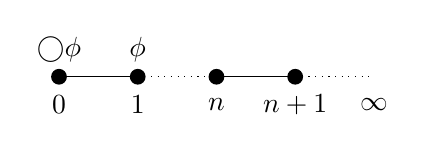
\begin{tikzpicture}
	\node at (0,0.35) (phi) {$\bigcirc\phi$};
	\node at (1,0.35) (phi) {$\phi$};
	\node at (1,-0.35) (1) {$1$};
	\node at (0,-0.35) (0) {$0$};
	\node at (2,-0.35) (n) {$n$};
	\node at (3,-0.35) (1) {$n+1$};
	\node at (4,-0.35) (1) {$\infty$};
	\fill (0,0) circle (0.1cm);
	\fill (1,0) circle (0.1cm);
	\fill (2,0) circle (0.1cm);
	\fill (3,0) circle (0.1cm);
	\path (0,0) edge (1,0) 
	(1,0) edge[dotted] (2,0)
	(2,0) edge (3,0)
	(3,0) edge[dotted] (4,0);
	\end{tikzpicture}
\end{center}
$\phi \mathcal{U}\psi$
به این معنی است که $\phi$ حداقل تا قبل از اینکه $\psi$ برقرار شود، برقرار است.( مثلا اگر بگوییم "تا وقتی که باران نباریده زمین خشک است" در این صورت "زمین خشک است" به جای $\phi$ و "باران باریده است" $\psi$ است).
\begin{center}
	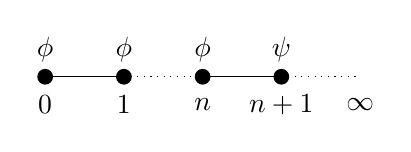
\begin{tikzpicture}
	\node at (1,0.35) (phi) {$\phi$};
	\node at (0,0.35) (phi) {$\phi$};
	\node at (2,0.35) (phi) {$\phi$};
	\node at (3,0.35) (phi) {$\psi$};
	\node at (1,-0.35) (1) {$1$};
	\node at (0,-0.35) (0) {$0$};
	\node at (2,-0.35) (n) {$n$};
	\node at (3,-0.35) (1) {$n+1$};
	\node at (4,-0.35) (1) {$\infty$};
	\fill (0,0) circle (0.1cm);
	\fill (1,0) circle (0.1cm);
	\fill (2,0) circle (0.1cm);
	\fill (3,0) circle (0.1cm);
	\path (0,0) edge (1,0) 
	(1,0) edge[dotted] (2,0)
	(2,0) edge (3,0)
	(3,0) edge[dotted] (4,0);
	\end{tikzpicture}
\end{center}

این زبان را می‌توان با ادوات بیشتری از آنچه آورده‌ایم بیان کرد و البته بیان‌های دیگری هم بسته به بحث متداول هستند، اما در اینجا یک شکل ساده از این زبان را آورده‌ایم که به غیر از ادوات منطق گزاره‌ای کلاسیک دو ادات دیگر را نیز دارد. دلیل وجود ادوات متفاوت، می‌تواند راحت‌تر کردن بیان ویژگی‌ها باشد. همان طور که استفاده نکردن از \gls*{disjunction} و \gls*{arrow} در منطق گزاره‌ای کلاسیک می‌تواند، به سخت کردن بیان جملات در چارچوب این منطق منجر شود، حذف این ادوات وجهی هم بیان ویژگی‌ها را در این منطق مشکل می‌سازد. 

حال که به درکی شهودی از معنای فرمول‌های این زبان رسیده‌ایم، به بیان صوری این مفاهیم می‌پردازیم.

\subsection{معناشناسی \lr{LTL}}

مدل‌های این منطق را به صورت \glspl*{function}
$M:\mathbb{N}_0 \rightarrow \mathit{P}(\Pi)$ 
تعریف می‌کنیم. به عبارت دیگر، هر مدل یک تابع است که هر \gls*{natnum} را به یک مجموعه از فرمول‌های اتمی می‌برد. این در واقع به این معنی است که یک مدل مشخص می‌کند که در هر لحظه کدام یک از فرمول‌های اتمی درست هستند. مثلا، در مدلی به نام $M$ در واقع
$M(5)$
مجموعه‌ی اتم‌هایی است که در لحظه‌ی 5 طبق این مدل درست هستند و اگر اتمی در این مجموعه حاضر نباشد، در لحظه‌ی 5، ارزش غلط دارد.
\gls*{truth} یک فرمول در یک مدل را با 
$M,i$
نشان می‌دهیم. 
$M,i \models \phi$
به این معنی است که فرمول $\phi$، در لحظه‌ی $i$ در مدل $M$ \gls*{true} است. این مفهوم را، به صورت \gls*{recursive}، به شکل زیر تعریف می‌کنیم:


\begin{flushleft}
$	M,i \models \pi \:\:\: \mathit{iff} \:\:\: \pi \in M(i),$\\
$	M,i \models \neg \phi \:\:\: \mathit{iff} \:\:\: M,i\nvDash \phi,$\\
$	M,i \models \phi \lor \psi \:\:\: \mathit{iff} \:\:\: M,i \models \phi \:\:\: \mathit{or} \:\:\: M,i \models \psi,$\\
	 $M,i \models \bigcirc \phi  \:\:\:  \mathit{iff} \:\:\: M,i+1 \models \phi,$\\
	 $M,i \models \phi \mathcal{U} \psi \:\:\: \mathit{iff} \:\:\: 
	 \exists k \geq i \in \mathbb{N}_0: \forall i\leq j< k: M,j \models \phi \:\:\: \mathit{and} \:\:\: M,k \models \psi.$
\end{flushleft}


یک فرمول را \gls*{satisfiable} می‌گوییم اگر و تنها اگر مدلی وجود داشته باشد که فرمول در آن درست باشد.
اگر یک فرمول در هر مدلی درست باشد، آن فرمول را \gls*{valid} می‌گوییم.\\



\section{نحو زبان مورد بررسی‬}
یا فرض اینکه $\mathbb{X}$ مجموعه‌ی همه‌ی متغیرهای این زبان باشد، نحو زبان بیان برنامه‌ها \gls*{subset}ای از نحو زبان \lr{C} است، به شکل زیر:
$$\mathsf{x,y},... \in \mathbb{X}\hspace{4.65cm}$$
$$\mathsf{A} \in \mathbb{A} ::=\mathsf{1\:|\:x\:|\:A_1 - A_2\hspace{2.4cm}}$$  
$$\mathsf{B \in \mathbb{B} ::=A_1<A_2 \:|\: B_1 \: nand\: B_2\hspace{1.2cm}}$$
$$\mathsf{E \in \mathbb{E}::= A \: | \: B\hspace{4cm}}$$
$$\mathsf{S\in \mathbb{S} ::=\hspace{5cm}  }$$
$$\mathsf{x\doteq A; \hspace{2.25cm}}$$
$$\mathsf{|\:\:\:;\hspace{3.75cm}}$$
$$\mathsf{|\:\:\:if\:(B)\:S\:|\:if\:(B)\:S\:else\:S}$$
$$\mathsf{|\:\:\:while\:(B)\:S\: | \: break;\hspace{0.65cm}}$$
$$\mathsf{|\:\:\:\{Sl\}\hspace{3.15cm}}$$
$$\mathsf{Sl \in \mathbb{SL}::=Sl\:\:\:S\:|\:\backepsilon}\hspace{3.05cm}$$
$$\mathsf{P\in \mathbb{P}\:::=Sl}\hspace{4.25cm}$$
به اعضای مجموعه‌ها‌ی
 $\mathbb{A}$،
 $\mathbb{B}$،
 $\mathbb{S}$،
 $\mathbb{Sl}$
 و
 $\mathbb{P}$
 به ترتیب
 \gls{aexp}، 
 \gls{boolexp}،
 \gls{statement}،
 \gls{statementlist} و
 \gls{program}
 می‌گوییم.\\

قابل مشاهده است که این زبان، نسبت به کل زبان \lr{C}، تا حد ممکن ساده‌سازی شده است. علت این کار را بعدا عمیق‌تر حس خواهیم‌کرد. علتْ ساده‌تر شدن کار برای ارائه‌ی معناشناسی و صورت‌های جدید روش وارسی مدل است. در اینجا، راحتی برنامه نوشتن در این زبان مطرح نبوده است، چون اصلا این زبان برای این کار ساخته نشده است. هدف از ارائه‌ی این زبان صرفا ارائه‌ی روش جدید است. یعنی می‌توان به این زبان به چشم یک \gls*{modelofcomputation}، مانند \gls{turingmachine} و \gls{registermachince} نگاه کرد. روشی که سعی در ارائه‌‌ی آن داریم، برای \glspl*{implang} است، مانند \gls{python}، \gls{java} و \lr{C}. بنابراین، انتخاب یک مدل محاسبه که رفتاری شبیه‌تر به این زبان‌ها داشته باشد، کار معقولی است.

اندکی در مورد \gls*{expressivity} این زبان صحبت می‌کنیم. می‌توانیم باقی اعداد را از روی عدد ۱ و \gls*{operator} \gls*{subtraction} بسازیم. مثلا ابتدا 0 را به کمک ۱-۱ می سازیم و سپس، با استفاده از 0 می‌توانیم یکی یکی \glspl*{negnum} را بسازیم. پس از آن، به سراغ \glspl*{posnum} می‌رویم که با کمک 0 و هر عدد صحیح منفی‌ای که ساخته‌ایم، ساخته می‌شوند. باقی اعداد و حتی عملگر‌ها( یعنی به غیر از اعداد طبیعی) از روی اعداد و عملگرهایی که داریم قابل‌ساختن هستند. در \glspl{boolexp} نیز با داشتن دسته‌‌ای محدود اما کافی از عملگر‌ها، باقی عملگر‌های رایج \gls*{expressible} هستند. یعنی اینجا صرفا \gls{shefferop} تعریف شده است و باقی \glspl{boolop}را می‌توان با استفاده از همین عملگر ساخت. باقی دستورات نیز دستورات \gls*{conditional} و \gls*{loop} هستند و مطابق رفتاری که از آن‌ها در زبان \lr{C} انتظار داریم، کار می‌کنند. در مورد دستور \lr{$\mathsf{break;}$} ذکر این نکته ضروری است که اجرای این دستور، اجرای برنامه را از دستوری بعد از داخلی‌ترین حلقه‌ای که \lr{$\mathsf{break;}$} داخلش قرار دارد، ادامه می‌‌دهد. در پایان می توان ثابت کرد که این زبان \gls*{equivalent} با ماشین تورینگ\cite{davis} است. 

هر‌آنچه بالاتر در‌مورد معنای دستورات این زبان گفتیم، به هیچ وجه صوری نبود. صرفا یک درک شهودی‌ که از معنای \gls*{execution}ی هر‌یک از دستورات می‌توان داشت را بیان کرده‌ایم. بیان صوری معنای برنامه‌ها را که قابل انتقال به کامپیوتر‌ است( خلاف درک شهودیمان)، در ادامه بیان خواهیم‌کرد. بدیهی است که یک بیان صوری از روی یک درک شهودی ساخته می‌شود، اما این دو استفاده‌های متفاوتی دارند.

\section{معناشناسی زبان مورد بررسی‬}
معناشناسی زبانی را که در بخش پیش آورده‌ایم، با کمک مفاهیمی به نام‌های \gls{label} و \gls{prefixtrace} و عملگری به نام \gls{concat} تعریف می‌کنیم. نام این معناشناسی، معناشناسی رد پیشوندی است.\\

\subsection{برچسب‌ها}

با‌وجود اینکه در نحو زبان \lr{C} برچسب‌ها وجود دارند،اما در نحو زبانی که معرفی کرده‌ایم، برچسب‌ها حضور ندارند. با این وجود، در تعریف معناشناسی صوری برای برنامه‌ها، به این مفهوم نیاز داریم. در این بخش، به ‌طور غیر دقیق معنای برچسب‌ها را آورده‌ایم. همین تعاریف غیر دقیق برای کار ما کافی است. تعاریف صوری دقیق‌تر برچسب‌ها در پیوست \cite{calcul} آورده‌شده‌اند. از آوردن مستقیم این تعاریف در اینجا خود‌داری کرده‌ایم. البته در مورد تعریف صوری برجسب‌ها، قابل ذکر است که طبق \cite{cousotbook}، تعریف صوری برچسب‌ها \gls*{nondeter} است(به عبارتی منفی نگرانه \gls*{welldef} نیست). به عبارت دیگر، تعریف‌های صوری مشخص‌تر متفاوتی را می‌توان متصور شد که در تعریف صوری برچسب‌ها در \cite{cousotbook} می‌گنجند.

در نحو زبانمان، \lr{$\mathsf{S}$}ها بخشی از \glspl*{expression}ی موجود در نحو زبان هستند که به آن‌ها \gls{statement} می‌گوییم. برچسب‌ها را برای \lr{$\mathsf{S}$}ها تعریف می‌کنیم. برچسب‌ها با کمک توابع \lr{labs, in, brks-of, brk-to, esc, aft, at} تعریف می‌شوند. در‌ واقع، هر $\mathsf{S}$، به ازای هر یک از این توابع، ممکن است یک برجسب متفاوت داشته باشد. بعضی دیگر از این توابع به ازای هر $\mathsf{S}$ ممکن است یک مجموعه از برچسب‌ها را برگردانند. یکی از آن‌ها هم با گرفتن $\mathsf{S}$ یک \gls{boolval} را بر‌می‌گرداند. 
\\\\
\lr{at$\llbracket\mathsf{S}\rrbracket$} : برچسب شروع $\mathsf{S}$.\\
\lr{aft$\llbracket\mathsf{S}\rrbracket$} : برچسب پایان $\mathsf{S}$، اگر پایانی داشته باشد.\\
\lr{esc$\llbracket\mathsf{S}\rrbracket$} : یک مقدار بولی را باز‌‌می‌گرداند که بسته به اینکه در $\mathsf{S}$ عبارت دستوری $\mathsf{break;}$ وجود دارد یا خیر، مقدار درست یا \gls*{false} را بر‌می‌گرداند.\\
\lr{brk-to$\llbracket\mathsf{S}\rrbracket$} : 
برچسبی است که اگر حین اجرای $\mathsf{S}$ عبارت دستوری $\mathsf{break;}$ اجرا شود، برنامه از آن برچسب ادامه پیدا می کند.\\
\lr{brks-of$\llbracket\mathsf{S}\rrbracket$} :
مجموعه‌ای از برچسب‌های عبارت‌های دستوری
$\mathsf{break;}$
که داخل $\mathsf{S}$ هستند را بر‌می‌گرداند.\\
\lr{in$\llbracket\mathsf{S}\rrbracket$} : مجموعه‌ای از تمام برچسب‌های درون $\mathsf{S}$ را برمی‌گرداند.\\
\lr{labs$\llbracket\mathsf{S}\rrbracket$} : مجموعه‌ای از تمام بر‌چسب‌هایی که با اجرای $\mathsf{S}$ قابل دسترسی هستند را بر‌می‌گرداند.\\\\\\
مجموعه‌ی همه‌ی برچسب‌ها را با 
$\mathbb{L}$
نشان می‌دهیم.

\subsection{رد پیشوندی}


حال که تعریف برچسب‌ها را داریم، به سراغ تعریف رد پیشوندی می‌رویم. البته پیش از آن، باید \gls{state}‌ و \gls{environment}‌ را تعریف کنیم.
\begin{defn}
	(محیط): به ازای مجموعه \glspl{value}
	 $\mathbb{V}$
	  و مجموعه \glspl{variable} 
	  $\mathbb{X}$ تابع 
	$\rho : \mathbb{X} \rightarrow \mathbb{V}$ 
	را یک محیط می‌گوییم. مجموعه‌ی همه‌ی محیط‌ها را با $\mathbb{EV}$ نمایش می‌دهیم.
\end{defn}

\begin{defn}
	(وضعیت): به هر \gls*{pair} متشکل از یک برچسب $l$ و یک محیط $\rho$ یک وضعیت  
	$\langle l , \rho \rangle$
	می‌گوییم. مجموعه‌ی همه‌ی وضعیت‌ها را با $\mathfrak{S}$ نشان می‌دهیم.
\end{defn}
\begin{defn}
	(رد پیشوندی): به یک \gls*{seq} از وضعیت‌ها( با امکان \gls*{empty} بودن) یک رد پیشوندی می‌گوییم.
\end{defn}

هر رد پیشوندی یک دنباله است که قرار است توصیفی از \gls{workflow} اجرای یک برنامه باشد. منظور از گردش کار این است که در هر لحظه، حافظه چه وضعیتی دارد و اینکه برنامه در حال اجرای چه دستوری است. وضعیت‌ها موقعیت لحظه‌ای \gls*{memory}ا‌ی که در دسترس برنامه است را توصیف می‌کنند. $l$ برچسب قسمتی از برنامه‌ است که در حال اجرا است و $\rho$ مقدار متغیر‌ها را در آن لحظه از اجرای برنامه نشان می‌دهد. ردهای پیشوندی می‌توانند \gls*{fin} یا \gls*{inf} باشند. مجموعه‌ی ردهای پیشوندی‌ متناهی را با $\mathfrak{S^+}$ و مجموعه‌ی ردهای پیشوندی نامتناهی را با  $\mathfrak{S^\infty}$ نمایش می‌دهیم. مجموعه‌ی همه‌ی ردهای پیشوندی را هم با $\mathfrak{S^{+\infty}}$ نمایش می‌دهیم. 
با توجه به آنچه گفتیم، یک عملگر چسباندن $\Join$ را روی ردهای پیشوندی تعریف می‌کنیم. 

پیش از ارائه‌ی تعریف، به دو نکته‌ی مهم در مورد نمادگذاری‌های این پایان نامه اشاره می‌کنیم.

اولین نکته این است که حین ارائه‌ی تعریف‌ها، مانند تعریف عملگر چسباندن که در ادامه آمده است، اگر تعریف را روی یک \gls*{structure} یا با در نظر گرفتن پیش‌فرض‌های مختلف ارائه داده باشیم، هر فرض را با علامت 
$\blacktriangleleft$
نشان داده‌ایم. در اثبات‌ها، برای هر \gls*{case} از 
$\blacktriangleright$
استفاده کرده‌ایم. اگر حین ارائه‌ی یک تعریف یا اثبات، پس از ارائه‌ی یک پیش‌فرض، احتیاج به پیش‌فرض بیشتری داشته باشیم، پیش‌فرض دومی را با $\blacktriangleleft\blacktriangleleft$ یا $\blacktriangleright\blacktriangleright$ نشان داده‌ایم. مثلا فرض کنید می‌خواهیم یک تابع به اسم $f$ روی اعداد صحیح تعریف کنیم، که به ازای ورودی‌های زوج، همان ورودی را برمی‌گرداند و اگر ورودی فرد باشد، اگر  عدد بر 3 بخش پذیر باشد، حاصل تقسیم آن را بر 3 برمی‌گرداند و اگر نباشد، باقی مانده‌ی آن را در تقسیم بر 3 برمی‌گرداند. تعریف این تابع با نمادگذاری‌ای که گفتیم، با فرض اینکه $n$ ورودی تابع و $k$ و $k'$ دو عدد صحیح باشند، به این شکل می‌شود:
$$\blacktriangleleft n=2k+1:$$
$$\blacktriangleleft\blacktriangleleft n=3k':$$
$$f(n)=k'$$
$$\blacktriangleleft\blacktriangleleft n=3k'+1:$$
$$f(n)=1$$
$$\blacktriangleleft\blacktriangleleft n=3k'+2:$$
$$f(n)=2$$
$$\blacktriangleleft n=2k:$$
$$f(n)=n$$
 یا اگر اعضای یک مجموعه‌ی دلخواه $K$ با ساختار 
 $k \in K ::= a | b$
 تعریف شود، تابع همانی $f$ را روی $K$ در این نمادگذاری به شکل زیر نشان می‌دهیم: 
$$\blacktriangleleft f(a)=a$$ 
$$\blacktriangleleft f(b)=b$$
 

نکته‌ی دوم در مورد نشان دادن ردهای پیشوندی است. اگر $\pi_1,\pi_2$ رد پیشوندی باشند و $\sigma$ یک وضعیت باشد، $\pi_1\sigma$ به یک رد پیشوندی لزوما متناهی اشاره می‌کند که با وضعیت $\sigma$ به پایان رسیده است،
$\sigma\pi_1$
به یک رد پیشوندی اشاره می‌کند که با وضعیت $\sigma$ شروع شده است و $\pi_1\pi_2$ به یک رد پیشوندی اشاره می‌کند که با $\pi_1$ شروع شده است و با $\pi_2$ ادامه پیدا می‌کند( $\pi_1$ باید متناهی باشد). توجه شود که $\pi_1\pi_2$ با چسباندن $\pi_1$ و $\pi_2$ $(\pi_1 \Join \pi_2)$به همدیگر متفاوت است. هنگامی که می‌گوییم رد پیشوندی $\pi$( یا موقعیت $\sigma$) به رد پیشوندی $\pi'$ اضافه شده است، به رد پیشوندی $\pi'\pi$( یا $\pi'\sigma$) اشاره می‌کنیم.

\begin{defn}
	(عملگر چسباندن): برای 
	$\pi_1 , \pi_2 \in \mathfrak{S^{+\infty}}$ 
	و
	  $\sigma_1 ,\sigma_2 \in \mathfrak{S}$
	داریم:
		$$\blacktriangleleft \pi_1 \in \mathfrak{S}^\infty:$$
		$$\pi_1 \Join \pi_2 = \pi_1$$
		$$\blacktriangleleft \pi_1 \in \mathfrak{S}^+:$$
		$$\blacktriangleleft \blacktriangleleft \sigma_1 = \sigma_2:$$
		$$\pi_1\sigma_1 \Join \sigma_2 \pi_2 = \pi_1 \sigma_1 \pi_2$$
		$$\blacktriangleleft \blacktriangleleft \sigma_1 \neq \sigma_2:$$
		در این حالت 
		$\pi_1 \Join \pi_2$
		تعریف نمی‌شود.
\end{defn}
همین طور، $\epsilon$ یک رد پیشوندی است که حاوی هیچ وضعیتی نیست. به عبارت دیگر، یک دنباله‌ی تهی است.

\subsection{معناشناسی رد پیشوندی}
در این بخش، دو تابع $\mathcal{A}$ و $\mathcal{B}$ را به ترتیب روی \glspl{aexp} و عبارت‌های بولی، یعنی $\mathsf{A}$ها و $\mathsf{B}$ها تعریف می‌کنیم، سپس با کمک آنها تابع $\mathcal{S^*}$ را روی  مجموعه‌ای از اجتماع معنای $\mathsf{S}$ها و $\mathsf{Sl}$ها تعریف می کنیم. به هر $\mathsf{Sl}$ \gls{statementlist} می‌گوییم. در نهایت، تعریف  $\mathcal{S^*}$ را می‌آوریم.


\begin{defn}
	(معنای عبارت‌های حسابی - تابع $\mathcal{A}$): تابع 
	$\mathcal{A}:\mathbb{A}\rightarrow (\mathbb{EV} \rightarrow \mathbb{V})$
	را به صورت بازگشتی روی ساختار 
	$\mathsf{A} \in \mathbb{A}$
	به شکل زیر تعریف می‌کنیم:
	$$\blacktriangleleft\mathcal{A\llbracket\mathsf{1}\rrbracket\rho = }1     $$
	$$\blacktriangleleft\mathcal{A\llbracket\mathsf{x}\rrbracket\rho = } \rho(\mathsf{x})          $$
	$$\blacktriangleleft\mathcal{A\llbracket\mathsf{A_1-A_2}\rrbracket\rho = }\mathcal{A\llbracket\mathsf{A_1}\rrbracket\rho }- \mathcal{A\llbracket\mathsf{A_2}\rrbracket\rho }       $$
	
\end{defn}

\begin{defn}
	(معنای عبارت‌های بولی - تابع $\mathcal{B}$): تابع 
	$\mathcal{B}: \mathbb{B} \rightarrow (\mathbb{EV} \rightarrow \mathbb{BOOL})$
	را به صورت بازگشتی روی ساختار 
	$\mathsf{B} \in \mathbb{B}$
	به شکل زیر تعریف می‌کنیم:
	
	\begin{center}
		اگر $\mathcal{A\llbracket\mathsf{A_1}\rrbracket\rho }$ کوچکتر از $\mathcal{A\llbracket\mathsf{A_2}\rrbracket\rho }$ باشد
		$\blacktriangleleft\mathcal{B\llbracket\mathsf{A_1<A_2}\rrbracket\rho = } True   \hspace{2cm}  $\\
		اگر $\mathcal{A\llbracket\mathsf{A_1}\rrbracket\rho }$ بزرگتر از $\mathcal{A\llbracket\mathsf{A_2}\rrbracket\rho }$ باشد
		$\blacktriangleleft\mathcal{B\llbracket\mathsf{A_1<A_2}\rrbracket\rho = } False   \hspace{2cm}  $\\
		$ \blacktriangleleft\mathcal{B\llbracket\mathsf{B_1 nand B_2}\rrbracket\rho = } \neg(\mathcal{B\llbracket\mathsf{B_1}\rrbracket\rho}   \wedge \mathcal{B\llbracket\mathsf{B_2}\rrbracket\rho}) $
	\end{center}

طبیعتا $\wedge$ و $\neg$ در فرازبان هستند. منظور این است که این دو، ادوات درون یک زبان صوری نیستند، بلکه عطف و فصل در زبانی هستند که در آن در حال ارائه‌ی همه‌ی این تعاریف هستیم.
\end{defn}

در ادامه، به تعریف $\mathcal{S^*}$ می‌پردازیم. این کار را با تعریف $\mathcal{S^*}$ روی هر ساختار عبارت دستوری $\mathsf{S}$، لیست عبارت دستوری $\mathsf{Sl}$ و برنامه‌ی $\mathsf{P}$ انجام می‌دهیم. یعنی دامنه‌ی $\mathcal{S}^*$ مجموعه‌ی $\mathbb{P}\cup \mathbb{Sl}\cup\mathbb{S}$ است.
پیش از ادامه‌ی بحث، باید این نکته را در‌ مورد علامت‌گذاری‌هایمان ذکر کنیم که منظور از $        \mathsf{S} ::= l \mathsf{break;}  $ این است که تاکید کرده‌ایم که $\mathsf{S}$ با برچسب $l$ شروع شده‌است، هرچند که همین طور که پیش‌تر گفته‌شد،   $l$ جزو زبان نیست.

\begin{defn}
	(معنای برنامه‌ها - تابع $\mathcal{S}^*$): 
	$$\blacktriangleleft\mathsf{S} = \mathsf{break;}\;:$$
	$$\mathcal{S^*} \llbracket\mathsf{S}\rrbracket = \{ \langle at\llbracket\mathsf{S}\rrbracket , \rho \rangle | \rho \in \mathbb{EV}       \} \cup     \{ \langle at\llbracket\mathsf{S}\rrbracket , \rho \rangle \langle brk-to\llbracket\mathsf{S}\rrbracket , \rho \rangle | \rho \in \mathbb{EV}       \}             $$   
	
	
	$$\blacktriangleleft\mathsf{S}=\mathsf{x\doteq A;}\;:$$
	$$\mathcal{S^*} \llbracket\mathsf{S}\rrbracket = \{ \langle at\llbracket\mathsf{S}\rrbracket , \rho \rangle | \rho \in \mathbb{EV}       \} \cup     \{ \langle at\llbracket\mathsf{S}\rrbracket , \rho \rangle \langle aft\llbracket\mathsf{S}\rrbracket , \rho[\mathsf{x}\leftarrow \mathcal{A}\llbracket\mathsf{A}\rrbracket\rho] \rangle | \rho \in \mathbb{EV}       \}             $$   
	
	$$\blacktriangleleft\mathsf{S}= \mathsf{if}  \mathsf{ (B) S_t}:$$
	$$\mathcal{S^*} \llbracket\mathsf{S}\rrbracket = \{ \langle at\llbracket\mathsf{S}\rrbracket , \rho \rangle | \rho \in \mathbb{EV}       \} \cup     \{ \langle at\llbracket\mathsf{S}\rrbracket , \rho \rangle \langle aft\llbracket\mathsf{S}\rrbracket , \rho \rangle | \mathcal{B}\llbracket\mathsf{B}\rrbracket \rho =False      \} 
	$$$$\cup    \{ \langle at\llbracket\mathsf{S}\rrbracket , \rho \rangle \langle at\llbracket\mathsf{S_t}\rrbracket , \rho \rangle 
	\pi | \mathcal{B}\llbracket\mathsf{B}\rrbracket \rho =True  \wedge   \langle  at\llbracket\mathsf{S_t}\rrbracket  , \rho \rangle \pi \in \mathcal{S} \llbracket\mathsf{S_t}\rrbracket    \}          $$ 
	
	
	$$\blacktriangleleft\mathsf{S} = \mathsf{if}  \mathsf{ \;(B)\;S_t\;else\;S_f}:$$
	$$\mathcal{S^*} \llbracket\mathsf{S}\rrbracket = \{ \langle at\llbracket\mathsf{S}\rrbracket , \rho \rangle | \rho \in \mathbb{EV}       \} $$$$\cup     \{ \langle at\llbracket\mathsf{S}\rrbracket , \rho \rangle \langle at\llbracket\mathsf{S_f}\rrbracket , \rho \rangle 
	\pi | \mathcal{B}\llbracket\mathsf{B}\rrbracket \rho =False  \wedge   \langle  at\llbracket\mathsf{S_f}\rrbracket  , \rho \rangle \pi \in \mathcal{S} \llbracket\mathsf{S_f}\rrbracket    \}  
	$$$$\cup    \{ \langle at\llbracket\mathsf{S}\rrbracket , \rho \rangle \langle at\llbracket\mathsf{S_t}\rrbracket , \rho \rangle 
	\pi | \mathcal{B}\llbracket\mathsf{B}\rrbracket \rho =True  \wedge   \langle  at\llbracket\mathsf{S_t}\rrbracket  , \rho \rangle \pi \in \mathcal{S} \llbracket\mathsf{S_t}\rrbracket    \}          $$ \\
	
	
	$$\blacktriangleleft\mathsf{Sl}=\backepsilon:$$
	$$\mathcal{S^*} \llbracket\mathsf{Sl}\rrbracket = \{ \langle at\llbracket\mathsf{Sl}\rrbracket , \rho \rangle | \rho \in \mathbb{EV}       \}        $$ \\
	
	$$\blacktriangleleft\mathsf{Sl} = \mathsf{Sl' \:\:\: S}:$$
	$$\mathcal{S^*} \llbracket\mathsf{Sl}\rrbracket = \mathcal{S^*} \llbracket\mathsf{Sl'}\rrbracket \cup( \mathcal{S^*} \llbracket\mathsf{Sl'}\rrbracket
	\Join \mathcal{S^*} \llbracket\mathsf{S}\rrbracket )      $$ \\
	که در آن اگر فرض کنیم 
	$\mathcal{S,S'}$
	دو مجموعه شامل ردهای پیشوندی هستند، آنگاه عملگر چسباندن 
	$(\Join)$
	روی آن‌ها به شکل زیر تعریف می‌شود:
	$$\mathcal{S}\Join \mathcal{S}' = \{\pi \Join \pi' | \pi \in \mathcal{S}\land\pi' \in \mathcal{S}'\land (\pi \Join \pi'\;is\; well-defined) \}$$
	
	
	$$\blacktriangleleft\mathsf{S} = \mathsf{while\;(B)\;S_b}:$$
	 در این حالت، ماجرا نسبت به حالات قبل اندکی پیچیده‌تر می‌شود.
	 
	تابعی به اسم $\mathcal{F} $ را تعریف خواهیم‌کرد که دو ورودی دارد. ورودی اول آن یک عبارت‌ دستوری حلقه است و ورودی دوم آن یک مجموعه است. به عبارتی دیگر، به ازای هر حلقه یک تابع $\mathcal{F} $  جداگانه تعریف می‌شود که مجموعه‌ای از ردهای پیشوندی را می گیرد و مجموعه‌ای دیگر از همین موجودات را بازمی‌گرداند. کاری که این تابع انجام می‌دهد، این است که یک دور عبارت‌های دستوری داخل حلقه را اجرا می کند و دنباله‌های جدید را از دنباله‌های قبلی می‌سازد. 
	
	معنای یک حلقه را \gls{lfp} این تابع در نظر می‌گیریم. در ادامه، تعریف $\mathcal{F} $ آمده است. با دیدن تعریف، می توان به دلیل این کار پی‌برد. ورودی‌ای که دیگر $\mathcal{F} $ روی آن اثر نکند، در دو حالت ممکن است اتفاق بیافتد. اولی این است که شرط حلقه برقرار نباشد. طبق تعریف $\mathcal{F} $،  می‌توانیم ببینیم که $\mathcal{F} $  در این حالت چیزی به ردهای پیشوندی اضافه نمی‌کند.حالت دوم این است که اجرای برنامه داخل حلقه به عبارت‌ دستوری $\mathsf{break;}$ برخورد کرده باشد که در این صورت وضعیتی به ته ردهای پیشوندی اضافه می‌شود که برچسبش خارج از مجموعه برچسب عبارت‌های دستوری حلقه است و همین اضافه کردن هر چیزی را به ته ردهای پیشوندی موجود، توسط $\mathcal{F} $  غیرممکن می‌کند. 
	
	بنابراین، \gls{fp} مفهوم مناسبی برای این است که از آن در تعریف صوری معنای حلقه استفاده شود. علت اینکه کوچکترین نقطه‌ثابت را به عنوان معنای حلقه در نظر می‌گیریم، این است که مطمئن هستیم، هر رد پیشوندی‌ای در نقطه‌ثابت موجود باشد، به گردش کار برنامه مرتبط است و ردهای پیشوندی اضافی و بی‌ربط به معنای برنامه، به آن وارد نمی‌شوند. برای درک بهتر این نکته می‌توان به این توجه کرد که با اضافه کردن وضعیت‌هایی کاملا بی‌ربط به گردش کار برنامه به ته رد‌های پیشوندی، که صرفا برچسب متفاوتی با آخرین وضعیت هر رد پیشوندی دارند، نقطه‌ثابت جدیدی ساخته‌ایم. پس اگر خودمان را محدود به انتخاب کوچکترین نقطه‌ثابت نکنیم، به توصیفات صوری خوبی از برنامه‌ها دست پیدا نخواهیم‌کرد. 
	
	در مورد نقطه‌ثابت این نکته باقی می‌ماند که چه‌ طور می‌توانیم مطمئن باشیم که چنین نقطه‌ثابتی وجود دارد. در این رابطه، باید گفت که مجموعه‌هایی که از ردهای پیشوندی تشکیل شده‌اند، با \gls*{relation}‌ی زیرمجموعه بودن یک \gls*{lattice} را تشکیل می‌دهند. چون تابع $\mathcal{S}^*$ \gls*{monotonic} است، بنا به \gls{tarski}\cite{tarski} برای تابع $\mathcal{S}^*$ کوچکترین نقطه‌ثابت وجود دارد. یک تابع به نام $lfp^\subseteq$ نیز داریم، که یک تابع از نوع 
	$\mathit{P}(\mathfrak{S^*})\rightarrow\mathit{P}(\mathfrak{S^*})$
	را به‌‌ عنوان ورود می‌گیرد، سپس کوچکترین نقطه‌ثابت این تابع را باز می‌گرداند.
	باقی تعاریف نیز به این شکل هستند:
	
	$$\mathcal{S^*} \llbracket\mathsf{S}\rrbracket = lfp^{\subseteq}\: \mathcal{F\llbracket\mathsf{S}\rrbracket},$$
	 $$\mathcal{F} \llbracket\mathsf{S}\rrbracket X= \{ \langle at\llbracket\mathsf{S}\rrbracket , \rho \rangle | \rho \in \mathbb{EV}       \} \cup $$
	$$  \{ \pi_2 \langle l ,\rho \rangle \langle aft\llbracket\mathsf{S}\rrbracket,\rho \rangle |  \pi_2 \langle l ,\rho \rangle \in X \wedge \mathcal{B}\llbracket\mathsf{B}\rrbracket\rho=False \wedge l= at\llbracket\mathsf{S}\rrbracket   \} \cup      $$
	$$  \{ \pi_2 \langle l ,\rho \rangle \langle at\llbracket\mathsf{S_b}\rrbracket,\rho \rangle \pi_3 |  \pi_2 \langle l ,\rho \rangle \in X \wedge \mathcal{B}\llbracket\mathsf{B}\rrbracket\rho=True \wedge$$$$  \langle at\llbracket\mathsf{S_b}\rrbracket,\rho \rangle \pi_3 \in  \mathcal{S} \llbracket\mathsf{S_b}\rrbracket   \wedge   l= at\llbracket\mathsf{S}\rrbracket  \}  $$\\
	
	$$\blacktriangleleft\mathsf{S} =;  \;:$$
	$$\mathcal{S^*} \llbracket\mathsf{S}\rrbracket = \{ \langle at\llbracket\mathsf{S}\rrbracket , \rho \rangle | \rho \in \mathbb{EV}       \} \cup     \{ \langle at\llbracket\mathsf{S}\rrbracket , \rho \rangle \langle aft\llbracket\mathsf{S}\rrbracket , \rho \rangle | \rho \in \mathbb{EV}       \}             $$  
	
	
	$$\blacktriangleleft\mathsf{S}=\{\mathsf{Sl}\}:$$
	$$\mathcal{S^*} \llbracket\mathsf{S}\rrbracket = \mathcal{S^*} \llbracket\mathsf{Sl}\rrbracket $$   \\
\end{defn}
در اینجا، تعریف معنای برنامه‌ها به پایان می‌رسد.

